El \ME~es el formalismo teórico-experimental que, hasta el día de hoy, describe con mayor precisión las partículas elementales y sus interacciones. Los mayores desarrollos que dieron forma al \ME~ se obtuvieron en la segunda mitad del siglo XX con el desarrollo de la Teoría Cuántica de Campos: formulación conjunta de la mecánica cuántica y la mecánica relativista, que es capaz de describir la aniquilación, creación, decaimientos e interacciones de las partículas fundamentales. Los modelos teóricos y observaciones experimentales construyeron una clasificación de las partículas en base a sus propiedades fundamentales como lo son la masa, la carga eléctrica, la carga de color y el espín. Dicha clasificación se muestra en la Fig. \ref{estandar}. 

%En el mundo atómico y subatómico se tratan los problemas con la mecánica cuántica y unido a esto las magnitudes de las energías que se manejan para escudriñar el mundo subnuclear requiere del uso de la mecánica relativista superior en complejidad a la mecánica newtoniana, entonces 

\subsection{Composición de la materia e interacciones fundamentales} 

Las partículas elementales están divididas en dos categorías según el valor de su espín en \fermiones ~ (espín semi-entero, para elementales $1/2$) y \bosones ~ (espín entero, para elementales $1$ menos el higgs con $0$), estos obedecen también a la \fermidirac ~ y la \boseeinstein, respectivamente, solo cumpliendo el \pauli ~ los primeros.

El \ME ~ describe la composición de la materia bariónica usando 6 quarks, 6 leptones (fermiones) y partículas mediadoras de las interacciones fundamentales conocidas (bosones), que son los fotones $\mathbf{\gamma}$ (interacción electromagnética), los gluones $\mathbf{g}$ (interacción fuerte) y las partículas $\mathbf{W}^\pm$ y $\mathbf{Z}$ (fuerza débil). 
El bosón de Higgs $\mathbf{H}$ tiene un papel fundamental en el mecanismo de Higgs el cual dota de la propiedad de masa a las partículas elementales. Actualmente la interacción gravitacional no está descrita por algún bosón del \ME.

\begin{figure}[!b]
    \centering
    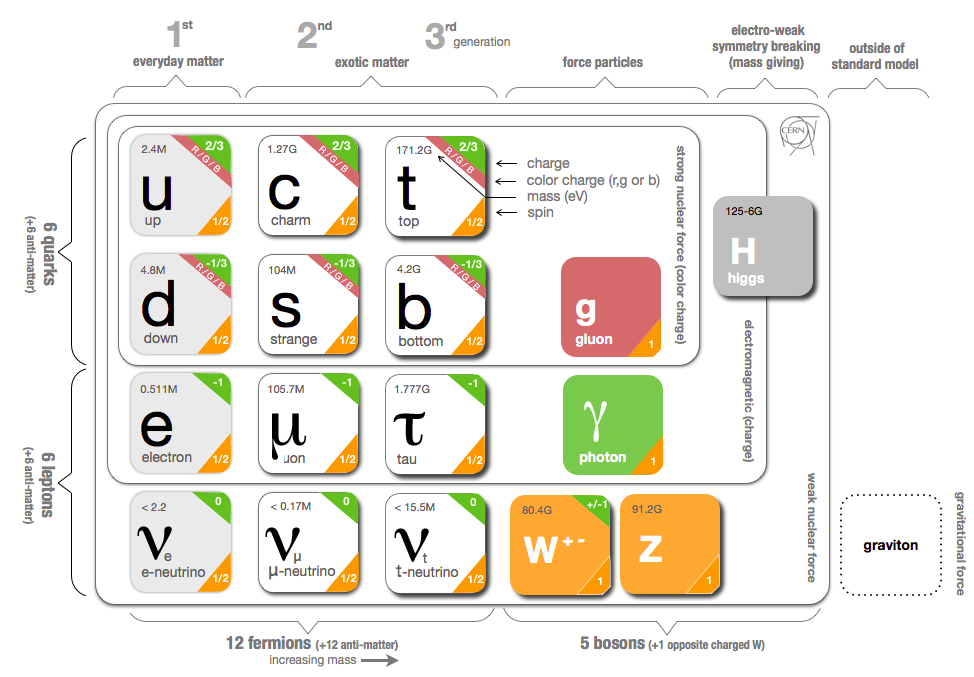
\includegraphics[width=.8\textwidth]{Fisica_de_Particulas/imagenes/standard_model.png}
    \caption{Clasificación de las partículas según el modelo estándar de las partículas elementales.}
    \label{estandar}
\end{figure}

%\subsection*{Quarks}

Los quarks Son fermiones que poseen carga eléctrica fraccionada ($- 1/3$ o $+ 2/3$) y carga de color (\textbf{R}, \textbf{G} o \textbf{B}), por lo que interactúan por medio del fotón $\gamma$ y del glúon $\mathbf{g}$. El campo de estudio dedicado a las interacciones entre quarks y gluones se llama Cromodinámica Cuántica (\QCD). Sin embargo, los quarks solo se encuentran en estados ligados llamados hadrones, ya sean bariones formados por tres quarks de diferente color (\textbf{qqq}), o mesones formado por un par quark-antiquark\footnote{Las antipartículas poseen la misma masa y espín, pero carga eléctrica contraria.} (\textbf{q\={q}}). Dado que los quarks son fermiones, dos quarks del mismo tipo no pueden tener los mismos n\'umeros cuánticos en el mismo hadrón.

En este grupo los quarks poseen carga eléctrica entera o neutra, estas son partículas indivisibles y por lo tanto elementales. Existen seis tipos como se pueden observar en la Fig. \ref{neuronas}: up $\mathbf{u}$(arriba), down $\mathbf{d}$(abajo), charm $\mathbf{c}$(encanto), strange $\mathbf{s}$(extrañeza), top $\mathbf{t}$(superior) y bottom $\mathbf{b}$(inferior). 
% ems: Nombrar los seis quarks haciendo referencia a la Fig. 1-1. Puedes poner de ejemplo a los dos bariones más conocidos: el neutrón y el protón.
Algunos ejemplos de bariones son:
\begin{itemize}
    \item \href{https://es.wikipedia.org/wiki/Bari\%C3\%B3n_omega}{\textbf{El neutrón ($N^0$) :}} es incluida en la definición de nucleones ya que conforman el núcleo de los átomos, es una partícula subatómica sin carga neta,  de la \QCD ~ se define que es partícula compuesta por la unión estable de quarks \textbf{udd}.
    \item \href{https://es.wikipedia.org/wiki/Prot\%C3\%B3n}{\textbf{El protón ($p^+$) :}} es incluida en la definición de nucleones ya que conforman el núcleo de los átomos, es una partícula subatómica con una carga eléctrica elemental positiva, de la \QCD ~ se define que es partícula compuesta por la unión estable \textbf{uud}.
\end{itemize}

Todos los hadrones tienen una respectiva antipartícula conformada por los antiquarks correspondientes.

%\subsection*{Leptones}

Los leptones forman parte de la familia de los fermiones por lo cual poseen espín semi-entero, además no poseen carga de color y por lo tanto tampoco experimentan la interacción nuclear fuerte. Se han identificado tres ``sabores'' de partículas, correspondientes al electrón $e$ y el neutrino $\nu_e$, al muón $\mu$ y el tauón $\tau$ con sus respectivos neutrinos $\nu_\mu$ y $\nu_\tau$ (ver Fig. \ref{estandar}).

\begin{itemize}
    \item \href{https://es.wikipedia.org/wiki/Electr\%C3\%B3n}{\textbf{El electrón :}} es una partícula elemental perteneciente a la primera generación de los leptones, representada por el símbolo $e^-$ posee una carga eléctrica elemental negativa. Su antipartícula es denominada positrón idéntica excepto por la carga de signo opuesto.
    
    \item \href{https://es.wikipedia.org/wiki/Muon}{\textbf{El muón :}} 
     es una partícula elemental masiva perteneciente a la segunda generación de leptones, representada por el símbolo $\mu^-$ su masa es 100 veces mayor que la del electrón. Su correspondiente antipartícula es el antimuón ($\mu^+$).
    
    \item \href{https://es.wikipedia.org/wiki/Tau_(part\%C3\%ADcula)}{\textbf{El tau :}} llamada a veces tauón, es una partícula elemental masiva que pertenece a la tercera generación de leptones, representada por el símbolo $\tau^-$, su masa es cerca de 3500 veces mayor que la del electrón. Su correspondiente antipartícula es el antitau o antitauón ($\tau^+$).
    
    \item \href{https://es.wikipedia.org/wiki/Neutrino}{\textbf{Los neutrinos :}}
    son partículas subatómicas sin carga y de espín $1/2$, que estas partículas tienen masa muy pequeña, su interacción con las demás partículas es mínima, por lo que pasan a través de la materia ordinaria sin apenas perturbarla. Existen tres tipos de neutrinos asociados a cada una de las familias leptónicas (o sabores): neutrino electrónico ($v_e$), neutrino muónico ($v_\mu$) y neutrino tauónico ($v_\tau$) más sus respectivas antipartículas.

\end{itemize}

Cada partícula anteriormente descrita con su correspondiente antipartícula corresponde con la composición de la materia bariónica.


\subsection{Simetrías y lagrangiano} 


Las teorías extensamente aceptadas del modelo estándar son referidas como teorías de campo de gauge y son la expresión de la existencia de alguna simetría interna haciendo que el lagrangiano $\mathcal{L}_{\mathbf{gauge}}$ sea invariante bajo la acción de un grupo de Lie\footnotetext{Son funciones diferenciables o analíticas que sirve para describir la simetría de estructuras analíticas, se clasifican por sus propiedades algebraicas, su conexidad y su compacidad.}, estás son referidas como grupo de transformaciones de gauge. De esta forma, al aplicar una transformación de gauge no se modifica ninguna propiedad física observable.

Los campos gauge aparecen en $\mathcal{L}_{\mathbf{gauge}}$ que rige la dinámica de los campos cuánticos. Éstos son: fermiónicos $\psi$, que representan a las partículas bariónicas; bosónicos electrodébiles $\mathbf{W_1}$, $\mathbf{W_2} $, $\mathbf{W_3}$ y $\mathbf{B}$; gluónicos $\mathbf{g}$; y el campo de Higgs $\varphi$ (ver Fig. \ref{simetrias}). Estos son definidos por operadores que no conmutan entre si y actúan sobre el estado cuántico del sistema. Además las partículas responsables de interacciones deben ser de masa cero ya que representan a simetrías de norma exactas y explícitas.
 
\begin{figure}[!t]
\centering
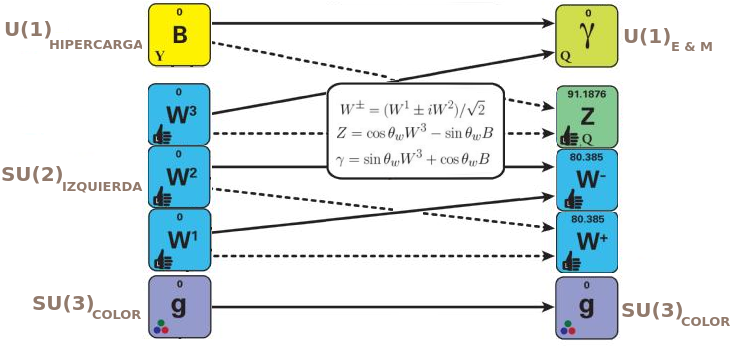
\includegraphics[width=1\textwidth]{Fisica_de_Particulas/imagenes/simetria0.png}
\caption[Simetrías del modelo estándar]{Simetrías del modelo estándar.\footnotemark}
\label{simetrias}
\end{figure}

%La dinámica del estado cuántico y los campos fundamentales están determinados por la densidad lagrangiana, que es además una teoría de gauge, de aquí que posea grados de libertad en el formalismo matemático que no se corresponden con los cambios en el estado físico este se corresponde con 
La lagrangiana del campo de gauge opera sobre el grupo dado por una simetría de norma $\mathbf{U(1) \otimes SU(2) \otimes SU(3)}$, donde $\mathbf{U(1)}$ actúa sobre $\mathbf{B}$ (interacción electromagnética) y $\mathbf{\varphi}$, $\mathbf{SU(2)}$ actúa sobre $\mathbf{W}$ y $\mathbf{\varphi}$ (interacciones débiles), y $\mathbf{SU(3)}$ actúa sobre $\mathbf{g}$ (interacciones fuertes entre los quarks en el espacio de color), por lo que de forma general todas las simetrías actúan sobre el campo fermiónico $\psi$.
La ruptura espontánea de esta simetría es uno de los ingredientes fundamentales de excitaciones de \href{https://es.wikipedia.org/wiki/Bos\%C3\%B3n\_de\_Goldstone}{Goldstone} que están asociadas a los términos de masa de los bosones de gauge, este es referido como mecanismo de Higgs.

%Aparte de los grupos de clasificación hay grupos que corresponden a ``simetrías espontáneamente rotas'', esto ocurre cuando estamos en un ``estado vacío'' que ya no es simétrico. 

%Siendo un hecho experimental el que las interacciones débiles (responsables de la radioactividad) son de muy corto alcance, deben ser entonces los mediadores de esta interacción de masa muy grande. Esto solo se concibe si la simetría de norma correspondiente a esta interacción está espontáneamente rota. Para que este fenómeno acontezca es necesario un ingrediente adicional en el modelo, este es el bosón de Higgs. 

El \ME ~ consiste entonces en un contenido de materia, los quarks y los leptones en tres familias, con una dinámica dictada por la simetría de norma $\mathbf{U(1) \otimes SU(2) \otimes SU(3)}$ y con un elemento adicional, el Higgs, responsable de la rotura (parcial) espontánea de  $\mathbf{U(1) \otimes SU(2)}$, fundamentada bajo la evidencia empírica de los resultados experimentales. El lagrangiano del modelo estándar que describe estas interacciones es:
\footnotetext{Página de origen: \href{https://en.wikipedia.org/wiki/Mathematical_formulation_of_the_Standard_Model}{https://en.wikipedia.org/wiki/Mathematical\_formulation\_of\_the\_Standard\_Model}}
\begin{equation}
\mathcal{L}_{\mathbf{SM}} = \mathcal{L}_{\mathbf{gauge}} + \mathcal{L}_{\mathbf{Fermion}} + \mathcal{L}_{\mathbf{Higgs}} + \mathcal{L}_{\mathbf{Yukawa}} + \mathcal{L}_{\mathbf{GF}} + \mathcal{L}_{\mathbf{Ghost}} 
\end{equation}
donde tenemos que:
\begin{itemize}

\item $\mathcal{L}_{\mathbf{gauge}}$ : resultado de la teoría de campo de calibración, esta resume la interacción entre fermiones como resultado de la introducción de transformaciones pertenecientes al grupo de simetría interna. %Esta transformación de gauge modifica un grado de libertad interno sin cambiar ninguna propiedad observable física. Esta transformación posee su respectivo campo de Yang-Mills asociado a las transformaciones y que describe la interacción física entre diferentes campos fermiónicos. Por ejemplo el campo electromagnético es un campo de gauge que describe el modo de interactuar de fermiones dotados con carga eléctrica. 
El lagrangiano de gauge describe la dinámica de los campos fermiónicos poseyendo alguna simetría interna ``local'' dada por un grupo de Lie, llamado grupo de transformaciones de gauge, transformando algún grado de libertad que no modifica ninguna propiedad física observable. %Las dos características formales que hacen de un campo un campo gauge son:
%\begin{itemize}
%\item Los campos gauge aparecen en el lagrangiano que rige la dinámica del campo en forma de conexión, por tanto, matemáticamente están asociadas a 1-formas que toman valores sobre una cierta álgebra de Lie.
%\item El campo de gauge puede ser visto como el resultado de aplicar a diferentes puntos del espacio diferentes transformaciones dentro del grupo de simetría asociado a los campos fermiónicos de la teoría.
%\end{itemize}
Su representación y desarrollo puede encontrarse en \cite{romao_resource_2012}.
%\begin{equation}
%\mathcal{L}_{gauge} = 
%-\dfrac{1}{4}G_{\mu v}^{a} G^{a\mu v} 
%-\dfrac{1}{4}W_{\mu v}^{a} W^{a\mu v} 
%-\dfrac{1}{4}B_{\mu v} B^{\mu v}
%\end{equation}

\item $\mathcal{L}_{\mathbf{Fermion}}$ : incluye los términos cinéticos para los fermiones, caracteriza la interacción con el gauge de campo debido a sus derivadas covariantes:
%\begin{equation}
%\mathcal{L}_{Fermion} = 
%\sum_{quarks} i \overline{q} \gamma^\mu D_\mu q +
%\sum_{\psi_L} i \overline{\psi_L} \gamma^\mu D_\mu \psi_L +
%\sum_{\psi_R} i \psi_R \gamma^\mu D_\mu \psi_R
%\end{equation}

%\item[-] $\mathcal{L}_{EW} = \mathcal{L}_{gauge} + \mathcal{L}_{Fermion}$ : El modelo electrodébil (\EW ~ de sus siglas en inglés) es aquella que unifica la interacción débil y el electromagnetismo (despreciando el primer término de los lagrangianos ya que están relacionados con la interacción de la fuerza fuerte y los \quarks), dos de las cuatro fuerzas fundamentales de la naturaleza, aplicada a todas las patículas del \ME, en esa teoría los fermiones son descritos mediante un lagrangiano de Dirac generalizado adecuadamente para que sea invariante gauge bajo un cierto grupo gauge de simetría interna. Teoricamente no existe una elección única de las simetrías del lagrangiano de las interacciones electrodébiles, estas son deducidas de resultados experimentales.
%
%De la evidencia experimental, se deduce que el grupo de simetría gauge mínimo capaz de acomodar las corrientes cargadas es \textbf{SU(2)}. La observación empírica ha permitido constatar que las interacciones \EW ~ actúan de manera distinta sobre los fermiones dextrógiros y sobre los fermiones levógiros constituye una de las características de este modelo. La aparición de esta simetría a partir de un lagrangiano originalmente simétrico es explicado formalmente por el mecanismo de ruptura espontánea de simetría.
%
%Por otro lado las fuerzas electromagnética y débil actúan sobre los mismos campos fermiónicos y no pueden ser descritas por separado, de aca que el grupo gauge mínimo que describe las interacciones electrodébiles es $\mathbf{U}(1)_Y \otimes \mathbf{SU}(2)_L$. Así, las corrientes cargadas de Yang-Mills incluyen solamente fermiones levógiros y no se conocen neutrinos dextrógiros. Es por ello que los campos fermiónicos levógiros son agrupados en dobletes, mientras que los campos dextrógiros son singletes del grupo $\mathbf{SU(2)_{L}}$ con simetría de isospín asociada con la conservación debil del mismo (donde el subíndice \textbf{L} únicamente indica la asimetría existente entre los fermiones de distinta helicidad), además la cantidad conservada por el grupo $\mathbf{U(1)_{Y}}$ es la hipercarga \textbf{Y}
%
%lo que quiere decir que las partículas son representantes de un grupo de gauge de tipo $\mathbf{U}(1)_Y \otimes \mathbf{SU}(2)_L$.

\item $\mathcal{L}_{\mathbf{Higgs}}$: describe el mecanismo de Higgs mediante el proceso que da masa a las partículas elementales, utiliza una teoría de gauge para dotar con masa a los bosones de gauge a través de la absorción de los bosones de Nambu–Goldstone derivados de la ruptura espontánea de simetría. %La implementación más simple del mecanismo agrega un campo de Higgs extra a la teoría de gauge. La ruptura espontánea de la simetría local subyacente desencadena la conversión de los componentes de este campo de Higgs a bosones de Goldstone que interactúan (al menos algunos de ellos) con los demás campos de la teoría, con el fin de producir términos de masas para (al menos algunos de) los bosones de gauge. 
%El sistema viene descrito por un Lagrangiano con la forma:
%\begin{equation}
%\mathcal{L}_{Higgs} = 
%(D_\mu \Phi)^\dagger D_\mu \Phi +
%\mu^2 \Phi^\dagger \Phi -
%\lambda (\Phi^\dagger \Phi)^2 = (D_\mu \Phi)^\dagger D_\mu \Phi - V(\Phi)
%\end{equation}
%donde $V(\Phi) \equiv \lambda (\Phi^\dagger \Phi)^2 - \mu^2 \Phi^\dagger \Phi$ conocido como el potencial renormalizable
\item $\mathcal{L}_{\mathbf{Yukawa}}$: describe el mecanismo de interacción entre un campo escalar y un campo de Dirac mediante una constante de acoplamiento. Su desarrollo se encuentra \citep{santamaria_masses_1993, romao_resource_2012}.
%\begin{equation}
%\mathcal{L}_{Yukawa} = -
%\overline{L_L} Y_L \Phi \ell_R -
%\overline{Q'_L} Y_d \Phi d'_R -
%\overline{Q'_L}Y_u \acute{\Phi}u'_R + h.c
%\end{equation}


%\item $\mathcal{L}_{GF}$: este se presenta como una elección matemática para hacer una elección en la teoría de los \textit{gauges} se realiza continuamente una elección constante, siendo este un procedimiento matemático para hacer frente a grados de libertad redundantes en las variables de campo. La mayoría de las predicciones físicas cuantitativas de una teoría de \textit{gauges} solo pueden obtenerse bajo una receta coherente para suprimir o ignorar estos grados de libertad no físicos. %La fijación juiciosa del \textit{gauge} puede simplificar enormemente los cálculos, pero se vuelve cada vez más difícil a medida que el modelo físico se vuelve más realista, esta es la forma tradicional de aplicación a la teoría cuántica de campos, la cual está llena de complicaciones relacionadas con la renormalización, especialmente cuando el cálculo continúa en órdenes superiores, de aquí que la búsqueda de procedimientos de obtención de \textit{gauges} lógicamente consistentes y manejables desde el punto de vista computacional, y los esfuerzos para demostrar su equivalencia frente a una variedad desconcertante de dificultades técnicas, ha sido un importante impulsor de la física matemática desde finales del siglo XIX hasta el presente. Su forma matemática tiene la forma:
%\begin{equation}
%\mathcal{L}_{GF} = - 
%\dfrac{1}{2\xi_G}F^2_G -
%\dfrac{1}{2\xi_A}F^2_A -
%\dfrac{1}{2\xi_Z}F^2_Z -
%\dfrac{1}{2\xi_W}F_-F_+
%\end{equation}
%su desarrollo se muestra en la sección 2.6 de la referencia \citep{romao_resource_2012}.

\item $\mathcal{L}_{\mathbf{Ghost}}$: %La última pieza necesaria el \ME ~ es el \LG, 
es una condición de fijación del medidor lineal haciendo uso de un campo adicional que se introduce en las teorías cuánticas de campos, de esta manera mantiene la consistencia de la formulación de integral del lagrangiano.%, esto es dado por la receta Fadeev-Popov.  La necesidad de fantasmas de Fadeev-Popov vino del requerimiento de que en la formulación de integral de caminos, las teorías cuánticas de campos deben proporcionar soluciones inequívocas, esto no es posible si una simetría de \textit{gauge} está presente ya que no hay ningún procedimiento para seleccionar ninguna solución a partir de una serie de soluciones físicamente equivalentes, todas relacionadas por una transformación de gauge. Su formulación matemática tiene la forma:
%\begin{eqnarray}
%\mathcal{L}_{Ghost}  = \eta_G \sum_{i=1}^4 \left[ 
%\overline{c_+} \dfrac{\partial(\delta F_+)}{\partial\alpha^i} +
%\overline{c_-} \dfrac{\partial(\delta F_-)}{\partial\alpha^i} +
%\overline{c_Z} \dfrac{\partial(\delta F_Z)}{\partial\alpha^i} +
%\overline{c_A} \dfrac{\partial(\delta F_A)}{\partial\alpha^i} +
%\right]c_i + \nonumber\\
%\eta_G \sum_{a,b=1}^8\overline{w}^a \dfrac{\partial(\delta F_G^a)}{\partial\beta^b} w^b 
%\end{eqnarray}
%
\end{itemize}


%Desde el punto de vista físico, los campos de gauge se manifiestan físicamente en forma de partículas bosónicas sin masa (bosones gauge), por lo que se dice que todos los campos de gauge son mediados por el grupo de bosones de gauge sin masa de la teoría.

% ems: cita el artículo sobre la observación del Higgs
El modelo estándar está respaldado por una serie de observaciones experimentales, la más reciente fue la observación de una nueva partícula cuyas propiedades son consistentes con el bosón de Higgs, sin embargo, aún existen fenómenos en la naturaleza que no pueden ser explicados dentro del formalismo del modelo estándar%, ejemplo de ello es la naturaleza y composición de la materia oscura
.

%Las interacciones se describen dentro del MS por medio de teorías de calibración (gauge) y se manifiestan a través del intercambio de partículas de espín entero (bosones). Las dos primeras interacciones (débil y electromagnética) están unificadas como se verá más adelante. No obstante la unificación de las tres fuerzas no se realiza dentro del MS, sino que se introducen tres constantes de acoplamiento (una por cada interacción). El marco matemático en el que se desarrolla el MS es la yustaposición de tres grupos de simetría: $ SU(3)_C \times SU(2)_L \times U(1)_Y$ . En la tabla \ref{BB100:tab:1.2} pueden verse los bosones gauge junto con las interacciones a las que están asociados y la fuerza relativa de cada una de estas.

%Las interacciones se describen dentro del MS por medio de teorías de calibración (gauge) y se manifiestan a través del intercambio de partículas de espín entero (bosones). Las dos primeras interacciones (débil y electromagnética) están unificadas como se verá más adelante. No obstante la unificación de las tres fuerzas no se realiza dentro del MS, sino que se introducen tres constantes de acoplamiento (una por cada interacción). El marco matemático en el que se desarrolla el MS es la yustaposición de tres grupos de simetría: $ SU(3)_C \times SU(2)_L \times U(1)_Y$ . En la tabla \ref{BB100:tab:1.2} pueden verse los bosones gauge junto con las interacciones a las que están asociados y la fuerza relativa de cada una de estas.

%\begin{table}
%  \begin{center}
%   \caption{Interacciones descritas por el Modelo Estándar junto con los grupos gauge y los bosones asociados a cada una de ellas. En la columna de la derecha 		se representan las constantes fundamentales que indican la fuerza relativa de cada interacción.}
%    \label{tab}
%    \begin{tabular}{|l|c|c|c|c|} % <-- Alignments: 1st column left, 2nd middle and 3rd right, with vertical lines in between
%		\hline 		
%		Interacción & Grupo calibración & Bosón & Símbolo & Fuerza relativa\\
%		\hline
%		Electromagnética & $U(1)$ & fotón & $\gamma$ & $\alpha_{em}= 1/137$\\
%		\hline
%		Débil & $SU(2)$ & bosones intermedios & $W^\pm$, $Z$ & $\alpha_{weak} = 1.02 \cdot 10^{-5}$\\
%		\hline
%		Fuerte & $ SU(3)$ & gluones (8 tipos) & $g$ & $\alpha_s{M_Z} = 0.121$\\
%		\hline
%    \end{tabular}
%  \end{center}
%\end{table}


\subsection{Insuficiencias del modelo}

Incluso cuando el \ME ~ ha tenido gran éxito en explicar disímiles resultados experimentales,  tiene ciertas cuestiones importantes sin resolver. Entre los problemas encontrados en la teoría estándar está la falta de explicación de los orígenes cuánticos de la gravedad haciendo que la teoría sea por el momento incompatible con la relatividad general. El \ME ~ solo puede explicar el 15.45\% de la material del universo y no considera posible la existencia de masa por parte de los neutrinos (cuestión refutada por los estudios de sus oscilaciones). No explica la presencia excesiva de materia que de antimateria, el modelo predice la creación y aniquilación en cantidades estadísticamente semejantes. Tiene \href{https://en.wikipedia.org/wiki/Hierarchy_problem}{problemas de jerarquía} al introducir partículas con masas a través del proceso de ``ruptura espontánea de simetría electrodébil'' (provocado por el campo de Higgs sobre la simetría de norma $\mathbf{U(1) \otimes SU(2)}$), forzando algunas correcciones cuánticas muy grandes debido a la presencia de partículas virtuales y mucho más grandes que la masa de Higgs real.


%\begin{itemize_f}
%\item[-] \textbf{Gravedad :} no 
%\item[-] \textbf{Materia oscura y energía oscura :} como se pudo constatar anteriormente, solo es posible explicar el 4.9\% de la materia presente en el universo. %Sobre el 95.1% que falta, aproximadamente 
%El 26.8\% de la materia del universo apenas interactúa con los campos del Modelo Estándar. %El resto debería ser energía oscura, una densidad de energía constante para el vacío. 
%Los intentos de explicar la energía oscura en términos de la energía del vacío del Modelo Estándar llevan a un error de 120 órdenes de magnitud.

%\item[-] \textbf{Masa de los neutrinos :} el \ME ~ considera a los neutrinos partículas sin masa, . % Los términos de masa para los neutrinos se pueden añadir a mano al Modelo Estándar, pero esto conduce a nuevos problemas teóricos. (Por ejemplo, los términos de masa deben ser extraordinariamente pequeños).

%\item[-] \textbf{Asimetría de la materia–antimateria :} el \ME ~ predice que la materia y la antimateria deben haber sido creadas en cantidades estadisticamente semejantes, cuestión que si fuera real hubiera aniquilado unas a otras durante el enfriamiento del universo.

%\item[-] \textbf{Problema de jerarquía : } teóricamente se introduce partículas con masas a través de un proceso de ruptura espontánea de simetría electrodébil provocado por el campo de Higgs. Dentro del modelo estándar, la masa de Higgs obtiene algunas correcciones cuánticas muy grandes debido a la presencia de partículas virtuales. Estas correcciones son mucho más grandes que la masa de Higgs real, consideración %. Esto significa que el parámetro de "Masa Desnuda" de Higgs en el modelo estándar debe ser ajustado de tal manera que cancele casi por completo las correcciones cuánticas. Este nivel de ajuste fino está considero como 
%no natural por muchos físicos teóricos.

%\item[-] \textbf{Problema CP fuerte :} teóricamente se puede argumentar que el modelo estándar debe contener un término que rompa la simetría \textbf{CP} (relacionando la materia con la antimateria), pero este no se ha encontrado.
%\item[-] 
%\item[-] 
%\end{itemize_f}
